\documentclass[11pt,a4paper]{scrartcl}
\typearea{12}
\usepackage{graphicx}
\usepackage{pstricks}
\usepackage{listings}

\usepackage{tikz}
\usepackage{tikzscale}
\usepackage{pgfplots}

\pgfplotsset{compat=1.8}


\lstset{language=python}
\pagestyle{headings}
\markright{Computational Neuroscience - 8 spike trains}
\begin{document}

\subsection*{Introduction}
These notes are about the analysis of spike trains. It is based on
Dayan \& Abbott, sections 1.2, 1.4 \& 3.2. There is also a set of
slides that go with this lecture containing pictures showing examples
from the literature where these methods have been used.

\subsection*{Decoding spike trains}
There are diverse methods for examining spike trains and describing or
decoding their activity; they are all useful in different ways and
unsatisfactory in others. The methods we will look at here will
typically involve histograms, that is, some sort of discretization of
time and \textsl{binning} of results; this is typically of the field.

\subsection*{Peristimulus time histogram}
The idea here is to look at the activity immediately after a
stimulus, so the stimulus is repeated as many times as is possible and
the spikes that occur different amounts of time after the stimulus are
binned together. Thus, a \textsl{trial} refers to the responses to a single presentation of the stimulus and
\begin{itemize}
\item Superimpose the trials with the stimulus times superposed.
\item Divide time into small intervals or bins.
\item Plot the spike count in each bin.
\end{itemize}
This is illustrated in Fig.~\ref{peri}. 

A related idea is the \textsl{spike triggered average}, this is used
when there is a continuous stimulus, such as the current level used to
stimulate an electric fish, and the spike triggered average shows the
average value of the stimulus at different amounts of time before a
spike. The spike triggered average can be interpreted in terms of the
sort of linear model we discussed in the case of vision. More
precisely, if there is a time dependent stimulus $s(t)$ and the $N$
spikes at times $t_i$ then the spike triggered average is
\begin{equation}
S(\tau)=\frac{1}{N}\sum_{i=1}^N s(t_i-\tau)
\end{equation}
In other words it gives the average amount of stimulus a time $\tau$
before a spike.

\begin{figure}
\begin{center}
\begin{tabular}{ll}
\textbf{a}&\\
&\includegraphics{peri_st.pgf}\\[1cm]
\textbf{b}&\\
&\includegraphics{peri_hist.pgf}
\end{tabular}
\end{center}
\caption{Peristimulus time histogram. \textbf{a} represents a spike
  train and stimulus, with the tall lines marking the stimulus and the
  short ones the spikes. \textbf{b} is the peristimulus time histogram
  with bin size 10 ms, we see that two spikes came within 1 ms of
  stimulus and five between 10 and 20 ms.\label{peri}}
\end{figure}

\subsection*{Autocorrelogram}
This shows how the behavior of a spike train is related to its
behavior at a different time; it is used to detect periodic behavior
in spike trains: a periodic spike train will have gaps between spikes
related to the period. To work out the autocorrelogram
\begin{itemize}
\item Divide time into small bins, of length $\delta t$ say. 
\item Count how many spikes are separated by a time between $n\delta
  t$ and $(n+1)\delta t$ and put them in the $n$th bin.
\item Plot the histogram.
\end{itemize}
This is illustrated in Fig.~\ref{auto}.

\begin{figure}
\begin{center}
\begin{tabular}{ll}
\textbf{a}&\\
&\includegraphics{auto_st.pgf}\\[1cm]
\textbf{b}&\\
&\includegraphics{auto_hist.pgf}
\end{tabular}
\end{center}
\caption{Autocorrelogram. \textbf{a} represents a spike train and
  \textbf{b} is the autocorrelogram. All spikes are a time distance of
  zero from themselves, so the central spike corresponds to the six
  spikes themselves.  The two for $\delta t=10$ ms tells us that there are
  two spikes that are one apart. This spike train is roughly periodic
  and that is matched by the behavior of the autocorrelogram where
  there are move spike pairs a distance 50 ms apart than, say 30 ms
  apart.\label{auto}}
\end{figure}

\subsection*{Cross correlogram}
A cross correlogram is useful for measuring the relationship between
the spiking in two neurons; it might give an indication that one
neuron may be influential in causing the other to spike or it might
show that both neurons are entrained to the same periodic behavior. It
is like the auto-correlogram except that it is gaps between spikes
from different spike trains that are measured and plotted. To work out the cross correlogram
\begin{itemize}
\item Divide time into small bins, of length $\delta t$ say. 
\item Count how many spikes from neuron two are found between $n\delta
  t$ and $(n+1)\delta t$ compared to the a spike from neuron one.
\item Plot the histogram.
\end{itemize}
This is illustrated in Fig.~\ref{cross}.


\begin{figure}
\begin{center}
\begin{tabular}{ll}
\textbf{a}&\\
&\includegraphics{cross_st2.pgf}\\[1cm]
\textbf{b}&\\
&\includegraphics{cross_hist.pgf}
\end{tabular}
\end{center}
\caption{Cross corellogram. \textbf{a} represents two spike train, one
  blue with spikes at 30, 90, 150, 160 and one yellow with spikes at 50, 110,
  120, 170, 180 and 190. \textbf{b} is the crosscorrelogram. These spike
  trains are both periodic in the same way, which shows up as the
  repeating bumps in the cross-correlogram and one fires just before
  the other, so, for example, the four in the 20 ms bin corresponds to
  the four yellow spikes that occur between 20 and 30 ms after a blue
  spike. This could indicate that one neuron is causing the other to
  fire, or that they are responding to the same overall periodicity,
  but with different lags.\label{cross}}
\end{figure}

\subsection*{Tuning curve}

The tuning curve is used to related the response to a family of
stimuli parameterized by a single variable, such as the angle of a bar
for vision. The tuning curve is a plot of the firing rate against the
parameter, so $r(\theta)$ for angle in vision. 

\subsection*{Decoding a single neuron}

Consider an experiment in which a monkey is shown a screen full of
moving dots, some move randomly but some move coherently to either the
left or right. The monkey is trained to move its eyes to the left if
the dots are moving that way and to right if that's the way the dots
are moving. If the monkey gets its detemination correct it gets a
treat, probably juice. The experimenter can control the coherence of
the dots, at one extreme there is no movement one way or another, all
the dots move randomly; at the other extreme all the dots are moving
the same way.

Britten et al. \cite{BrittenEtAl1992} managed to record from
a direction selective neuron in the monkey brain. Such a neuron has a
prefered direction. If the dots were moving the neurons preferred
direction it has a high firing rate, if they weren't, it has a low
one. However, in this noisy situation the firing rate varied from
trial-to-trial, the main thing is that the average is higher for
trials in the preferred direction to the other direction. In short, it
looks like there are two normal curves, one corresponding to the
preferred direction, the other to the other; these curves overlap and
overlap more and more as the coherence is lowered, making the motion
more random.

One way of describing how different the two distributions are is to
use $d'$. If $\mu_1$ is the average firing rate in the unpreferred
direction and $\mu_2$ in the preferred direction and assuming both
distributions have the same variance, then
\begin{equation}
d'=\frac{\mu_2-\mu_1}{\sigma}
\end{equation}
This is illustrated in Fig.~\ref{discrim}.

As an example, imagine that when the dots move left the firing rates
are $\{15,20,25\}$ and when they move right they are
$\{24,30,36\}$. Hence
\begin{equation}
\mu_1=\frac{15+20+25}{3}=20
\end{equation}
and
\begin{equation}
\mu_2=\frac{24+30+36}{3}=30
\end{equation}
Now, these data don't have the same variances, so we assume the
underlying distributions have the same variance and we average to
estimate this variance, so, using the unbiased estimator of the population average
\begin{equation}
\sigma^2=\frac{\sum_i(x_i-\mu)^2}{n-1}
\end{equation}
where there are $n$ data points $\{x_1,x_2,\ldots,x_n\}$, we get
\begin{equation}
\sigma_1^2=\frac{5^2+5^2}{2}=25
\end{equation}
and
\begin{equation}
\sigma_2^2=\frac{6^2+6^2}{2}=36
\end{equation}
hence $\sigma^2=30.5$. So
\begin{equation}
d'=\frac{30-20}{\sqrt{30.5}}=1.81
\end{equation}

\begin{figure}
\begin{center}
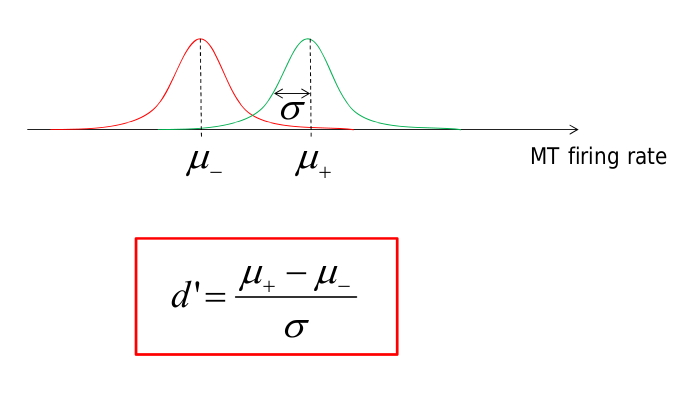
\includegraphics[width=10cm]{discrim.png}
\end{center}
\caption{Two different responses from an MT neuron. The green curve
  corresponds to the distribution of firing rate responses for the
  preferred direction, the red curve for the other one. $d'$ measures
  how different they are; it is basically the distance between the two
  means measured in units of the variance. [This figure was copied
  from Rafal's original slides.]\label{discrim}}
\end{figure}

This situation can be examined from the point-of-view of an ideal
observer, one who can't see the dots, but can see the firing rate of
two neurons, these are imagined as identical neurons except one
prefers left and the other prefers right. How well would this ideal
observer do trying to guess which way the dots are going? Imagine the
distribution of firing rates are normal so, say for the cell
preferring left if the dots are moving left the firing rate is chosen
randomly from $\mathcal{N}(\mu_2,\sigma)$ and if the dots are moving
right the firing rate is from $\mathcal{N}(\mu_1,\sigma)$. The other
neuron, the one which prefers right, is the same, but the other way
around. The idea observer has to then guess the neuron with the higher
firing rate is the one whose preferred direction is the one the dots
are moving in.

It is easy enough to calculate the chance the ideal observer would
come to the correct conclusion based on the firing rates, usually the
correct neuron has a higher firing rate than the rate for the other,
incorrect, neuron. Lets say the dots are going left, the probability
the observer is correct is the probability that the number chosen from
the right-preferring neuron (r) is higher than the one from the left-preferring
neuron (l). It is
\begin{equation}
P(\mbox{correct})=P[(\mbox{spikes from r neuron})>(\mbox{spikes from l neuron})]
\end{equation}
or, putting in the distributions
\begin{equation}
P(\mbox{correct})=P(\mathcal{N}(\mu_+,\sigma)>\mathcal{N}(\mu_-,\sigma))
\end{equation}
which, using the rules governing normal distributions
\begin{equation}
P(\mbox{correct})=P(\mathcal{N}(\mu_+-\mu_-,\sqrt{2}\sigma)>0)
\end{equation}
and, again using the identities for normal distributions this means
\begin{equation}
P(\mbox{correct})=P(\mathcal{N}(0,1)<\frac{\mu_+-\mu_-}{\sqrt{2}\sigma})
\end{equation}
By some algebra it turns out
\begin{equation}
P(\mbox{correct})=\Phi(d'/\sqrt{2})
\end{equation}
where $\Phi(t)$ is the cumulative for the normal distribution:
\begin{equation}
\Phi(t)=\int_{-\infty}^{t}p(\tau)d\tau
\end{equation}
where
\begin{equation}
p(\tau)=\frac{1}{\sqrt{2\pi}}e^{-\tau^2/2}
\end{equation}
is the probability mass function for $\mathcal{N}(0,1)$. It
starts at zero, for low $d'$ where it is very hard to distinguish it is near a half, and rises
to one for large $d'$, which is when you would expect it to be easy to
distinguish. In fact, in the Britten et al. paper
\cite{BrittenEtAl1992} they show that this curve matches the actual,
observed, behavior curves for how often the monkey made mistakes.

\begin{thebibliography}{10}

\bibitem{BrittenEtAl1992} 
Britten KH, Shadlen MN, Newsome WT, Movshon JA (1992). The analysis of visual motion: a comparison of neuronal and psychophysical performance. 
\newblock The Journal of Neuroscience, 12, 4745-4765.

\end{thebibliography}

\end{document}

